\documentclass[main.tex]{subfiles}

\usepackage{tikz}
\usetikzlibrary{automata,positioning}

\begin{document}


\tikzset{every picture/.style={line width=0.75pt}} %set default line width to 0.75pt        

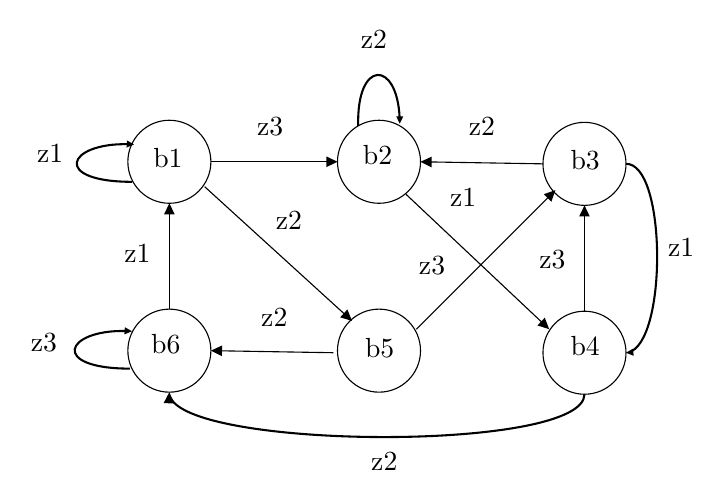
\begin{tikzpicture}[x=0.75pt,y=0.75pt,yscale=-1,xscale=1]
%uncomment if require: \path (0,300); %set diagram left start at 0, and has height of 300

%Shape: Circle [id:dp38007187440488943] 
\draw   (160,100) .. controls (160,88.95) and (168.95,80) .. (180,80) .. controls (191.05,80) and (200,88.95) .. (200,100) .. controls (200,111.05) and (191.05,120) .. (180,120) .. controls (168.95,120) and (160,111.05) .. (160,100) -- cycle ;
%Shape: Circle [id:dp21461313128983872] 
\draw   (261,100) .. controls (261,88.95) and (269.95,80) .. (281,80) .. controls (292.05,80) and (301,88.95) .. (301,100) .. controls (301,111.05) and (292.05,120) .. (281,120) .. controls (269.95,120) and (261,111.05) .. (261,100) -- cycle ;
%Shape: Circle [id:dp15383189343343084] 
\draw   (360,101) .. controls (360,89.95) and (368.95,81) .. (380,81) .. controls (391.05,81) and (400,89.95) .. (400,101) .. controls (400,112.05) and (391.05,121) .. (380,121) .. controls (368.95,121) and (360,112.05) .. (360,101) -- cycle ;
%Shape: Circle [id:dp8159389162470678] 
\draw   (160,191) .. controls (160,179.95) and (168.95,171) .. (180,171) .. controls (191.05,171) and (200,179.95) .. (200,191) .. controls (200,202.05) and (191.05,211) .. (180,211) .. controls (168.95,211) and (160,202.05) .. (160,191) -- cycle ;
%Shape: Circle [id:dp49070376813976546] 
\draw   (261,191) .. controls (261,179.95) and (269.95,171) .. (281,171) .. controls (292.05,171) and (301,179.95) .. (301,191) .. controls (301,202.05) and (292.05,211) .. (281,211) .. controls (269.95,211) and (261,202.05) .. (261,191) -- cycle ;
%Shape: Circle [id:dp782176541752861] 
\draw   (360,192) .. controls (360,180.95) and (368.95,172) .. (380,172) .. controls (391.05,172) and (400,180.95) .. (400,192) .. controls (400,203.05) and (391.05,212) .. (380,212) .. controls (368.95,212) and (360,203.05) .. (360,192) -- cycle ;
%Straight Lines [id:da7892663720759516] 
\draw    (200,100) -- (258,100) ;
\draw [shift={(261,100)}, rotate = 180] [fill={rgb, 255:red, 0; green, 0; blue, 0 }  ][line width=0.08]  [draw opacity=0] (5.36,-2.57) -- (0,0) -- (5.36,2.57) -- cycle    ;
%Curve Lines [id:da7808654548094007] 
\draw [line width=0.75]    (380,212) .. controls (380,239.65) and (192.82,238.76) .. (180.62,213.81) ;
\draw [shift={(180,211)}, rotate = 92.07] [fill={rgb, 255:red, 0; green, 0; blue, 0 }  ][line width=0.08]  [draw opacity=0] (5.36,-2.57) -- (0,0) -- (5.36,2.57) -- cycle    ;
%Straight Lines [id:da6171916688523531] 
\draw    (294,115.66) -- (360.82,178.6) ;
\draw [shift={(363,180.66)}, rotate = 223.29] [fill={rgb, 255:red, 0; green, 0; blue, 0 }  ][line width=0.08]  [draw opacity=0] (5.36,-2.57) -- (0,0) -- (5.36,2.57) -- cycle    ;
%Straight Lines [id:da980104563754469] 
\draw    (380,172) -- (380,124) ;
\draw [shift={(380,121)}, rotate = 90] [fill={rgb, 255:red, 0; green, 0; blue, 0 }  ][line width=0.08]  [draw opacity=0] (5.36,-2.57) -- (0,0) -- (5.36,2.57) -- cycle    ;
%Straight Lines [id:da5060478973614806] 
\draw    (360,101) -- (304,100.05) ;
\draw [shift={(301,100)}, rotate = 0.97] [fill={rgb, 255:red, 0; green, 0; blue, 0 }  ][line width=0.08]  [draw opacity=0] (5.36,-2.57) -- (0,0) -- (5.36,2.57) -- cycle    ;
%Straight Lines [id:da6569656708905764] 
\draw    (299,180.66) -- (363.88,115.78) ;
\draw [shift={(366,113.66)}, rotate = 135] [fill={rgb, 255:red, 0; green, 0; blue, 0 }  ][line width=0.08]  [draw opacity=0] (5.36,-2.57) -- (0,0) -- (5.36,2.57) -- cycle    ;
%Straight Lines [id:da042950844680829325] 
\draw    (180,171) -- (180,123) ;
\draw [shift={(180,120)}, rotate = 90] [fill={rgb, 255:red, 0; green, 0; blue, 0 }  ][line width=0.08]  [draw opacity=0] (5.36,-2.57) -- (0,0) -- (5.36,2.57) -- cycle    ;
%Straight Lines [id:da07906843129296459] 
\draw    (259,192) -- (203,191.05) ;
\draw [shift={(200,191)}, rotate = 0.97] [fill={rgb, 255:red, 0; green, 0; blue, 0 }  ][line width=0.08]  [draw opacity=0] (5.36,-2.57) -- (0,0) -- (5.36,2.57) -- cycle    ;
%Straight Lines [id:da6040560026037274] 
\draw    (197,112) -- (265.78,174.64) ;
\draw [shift={(268,176.66)}, rotate = 222.32] [fill={rgb, 255:red, 0; green, 0; blue, 0 }  ][line width=0.08]  [draw opacity=0] (5.36,-2.57) -- (0,0) -- (5.36,2.57) -- cycle    ;
%Curve Lines [id:da9537726518918423] 
\draw [line width=0.75]    (400,101) .. controls (419,100.67) and (419.95,181.88) .. (402.85,191.16) ;
\draw [shift={(400,192)}, rotate = 356.16] [fill={rgb, 255:red, 0; green, 0; blue, 0 }  ][line width=0.08]  [draw opacity=0] (3.57,-1.72) -- (0,0) -- (3.57,1.72) -- cycle    ;
%Curve Lines [id:da6082348937355344] 
\draw [line width=0.75]    (161,199.66) .. controls (122.2,199.66) and (129.5,180.84) .. (159.18,181.53) ;
\draw [shift={(162,181.66)}, rotate = 183.58] [fill={rgb, 255:red, 0; green, 0; blue, 0 }  ][line width=0.08]  [draw opacity=0] (3.57,-1.72) -- (0,0) -- (3.57,1.72) -- cycle    ;
%Curve Lines [id:da45421585922311203] 
\draw [line width=0.75]    (162,109.66) .. controls (123.2,109.66) and (130.5,90.84) .. (160.18,91.53) ;
\draw [shift={(163,91.66)}, rotate = 183.58] [fill={rgb, 255:red, 0; green, 0; blue, 0 }  ][line width=0.08]  [draw opacity=0] (3.57,-1.72) -- (0,0) -- (3.57,1.72) -- cycle    ;
%Curve Lines [id:da40805738209259057] 
\draw [line width=0.75]    (271,82.66) .. controls (270.03,50.65) and (289.76,50.63) .. (290.94,78.95) ;
\draw [shift={(291,81.66)}, rotate = 270] [fill={rgb, 255:red, 0; green, 0; blue, 0 }  ][line width=0.08]  [draw opacity=0] (3.57,-1.72) -- (0,0) -- (3.57,1.72) -- cycle    ;

% Text Node
\draw (171,92) node [anchor=north west][inner sep=0.75pt]   [align=left] {b1};
% Text Node
\draw (272,91) node [anchor=north west][inner sep=0.75pt]   [align=left] {b2};
% Text Node
\draw (372,93) node [anchor=north west][inner sep=0.75pt]   [align=left] {b3};
% Text Node
\draw (372,183) node [anchor=north west][inner sep=0.75pt]   [align=left] {b4};
% Text Node
\draw (273,184) node [anchor=north west][inner sep=0.75pt]   [align=left] {b5};
% Text Node
\draw (170,182) node [anchor=north west][inner sep=0.75pt]   [align=left] {b6};
% Text Node
\draw (115,90.66) node [anchor=north west][inner sep=0.75pt]   [align=left] {z1};
% Text Node
\draw (157,138.66) node [anchor=north west][inner sep=0.75pt]   [align=left] {z1};
% Text Node
\draw (112,181.66) node [anchor=north west][inner sep=0.75pt]   [align=left] {z3};
% Text Node
\draw (221,77.66) node [anchor=north west][inner sep=0.75pt]   [align=left] {z3};
% Text Node
\draw (230,122.66) node [anchor=north west][inner sep=0.75pt]   [align=left] {z2};
% Text Node
\draw (223,169.66) node [anchor=north west][inner sep=0.75pt]   [align=left] {z2};
% Text Node
\draw (276,238.66) node [anchor=north west][inner sep=0.75pt]   [align=left] {z2};
% Text Node
\draw (271,35.66) node [anchor=north west][inner sep=0.75pt]   [align=left] {z2};
% Text Node
\draw (299,144.66) node [anchor=north west][inner sep=0.75pt]   [align=left] {z3};
% Text Node
\draw (323,77.66) node [anchor=north west][inner sep=0.75pt]   [align=left] {z2};
% Text Node
\draw (314,111.66) node [anchor=north west][inner sep=0.75pt]   [align=left] {z1};
% Text Node
\draw (357,141.66) node [anchor=north west][inner sep=0.75pt]   [align=left] {z3};
% Text Node
\draw (419,135.66) node [anchor=north west][inner sep=0.75pt]   [align=left] {z1};


\end{tikzpicture}


\end{document}